
% This LaTeX was auto-generated from MATLAB code.
% To make changes, update the MATLAB code and republish this document.











    
    \begin{DoxyCode}
function example_jakstat_adjoint()

    % compile the model
    [exdir,~,~]=fileparts(which('example_jakstat_adjoint.m'));
    amiwrap('model_jakstat','model_jakstat_adjoint_syms',exdir)

    num = xlsread(fullfile(exdir,'pnas_data_original.xls'));

    D.t = num(:,1);
    D.condition= [1.4,0.45];
    D.Y = num(:,[2,4,6]);
    D.Sigma_Y = NaN(size(D.Y));
    D = amidata(D);

    xi =  [0.60
        3
        -0.95
        -0.0075
        0
        -2.8
        -0.26
        -0.075
        -0.41
        -5
        -0.74
        -0.64
        -0.11
        0.027
        -0.5
        0
        -0.5];

    options.sensi = 0;
    sol = simulate_model_jakstat([],xi,[],D,options);

    figure
    for iy = 1:3
        subplot(2,2,iy)
        plot(D.t,D.Y(:,iy),'rx')
        hold on
        plot(sol.t,sol.y(:,iy),'.-')
        xlim([0,60])
        xlabel('t')
        switch(iy)
            case 1
                ylabel('pStat')
            case 2
                ylabel('tStat')
            case 3
                ylabel('pEpoR')
        end
        ylim([0,1.2])
    end
    set(gcf,'Position',[100 300 1200 500])

    % generate new
    xi_rand = xi + 0.1;
    options.sensi = 1;
    options.sensi_meth = 'adjoint';
    sol = simulate_model_jakstat([],xi_rand,[],D,options);

    options.sensi = 0;
    eps = 1e-4;
    fd_grad = NaN(length(xi),1);
    for ip = 1:length(xi)
        xip = xi_rand;
        xip(ip) = xip(ip) + eps;
        psol = simulate_model_jakstat([],xip,[],D,options);
        fd_grad(ip) = (psol.llh-sol.llh)/eps;
    end

    figure
    scatter(abs(sol.sllh),abs(fd_grad))
    set(gca,'XScale','log')
    set(gca,'YScale','log')
    xlim([1e-2,1e2])
    ylim([1e-2,1e2])
    box on
    hold on
    axis square
    plot([1e-2,1e2],[1e-2,1e2],'k:')
    xlabel('adjoint sensitivity absolute value of gradient element')
    ylabel('finite difference absolute value of gradient element')
    set(gcf,'Position',[100 300 1200 500])


    drawnow

end
\end{DoxyCode}

         \begin{DoxyCode}Generating model struct ...
Parsing model struct ...

Generating C code ...
headers | wrapfunctions | 
Compiling mex file ...
amici | Building with 'Xcode with Clang'.
MEX completed successfully.
Building with 'Xcode with Clang'.
MEX completed successfully.
\end{DoxyCode} 
    
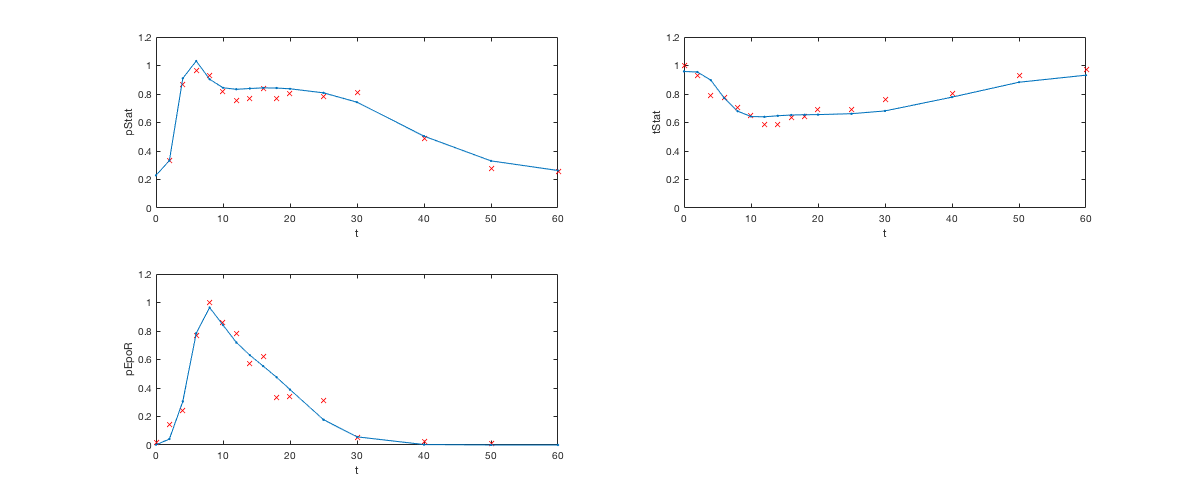
\includegraphics[width=\textwidth]{../../examples/example_jakstat_adjoint/html/example_jakstat_adjoint_01.png}

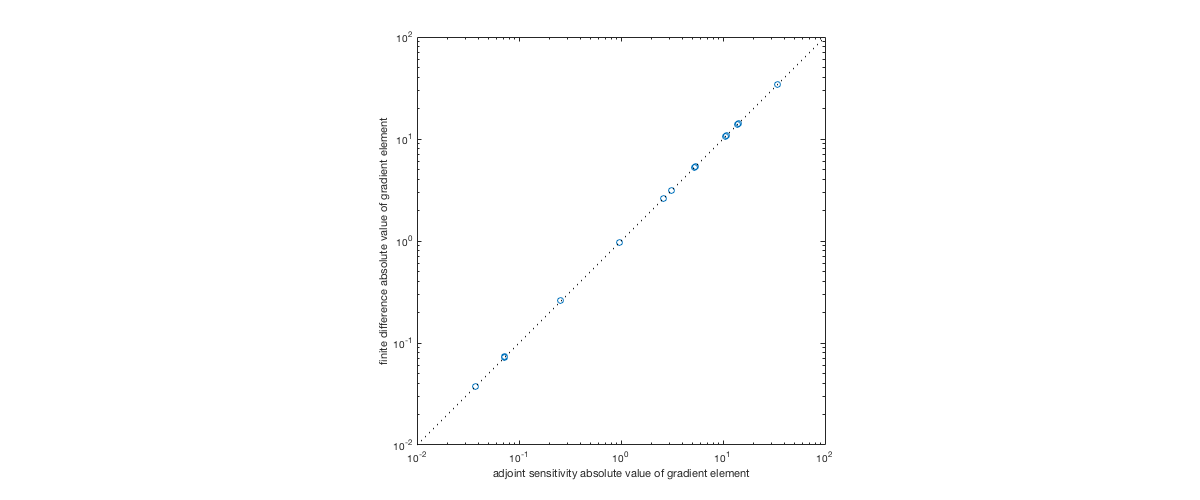
\includegraphics[width=\textwidth]{../../examples/example_jakstat_adjoint/html/example_jakstat_adjoint_02.png}




    